\documentclass[journal,12pt,twocolumn]{IEEEtran}
\usepackage{graphicx}
\graphicspath{{./images/}}
\usepackage{amsmath,amssymb,amsfonts,amsthm}
\newcommand{\myvec}[1]{\ensuremath{\begin{pmatrix}#1\end{pmatrix}}}
\usepackage{listings}
\usepackage{watermark}
\usepackage{titlesec}
\let\vec\mathbf
\lstset{
frame=single, 
breaklines=true,
columns=fullflexible
}
\thiswatermark{\centering \put(0,-105.0){
\includegraphics[scale=0.2]{logo2.png}} }
\title{\mytitle}
\title
{
Matrix Assignment - Circle
}
\author{Surajit Sarkar}
\begin{document}
\maketitle
\tableofcontents
\bigskip


\section{\textbf{Problem}}
If a circle passes through the point (a,b) and cuts the circle $x^2+y^2=p^2$ orthogonally, then the equation of the locus of its centre is 


\section{\textbf{Construction}}
 \begin{tabular}{|c|c|c|}
    \hline
    \textbf{Symbol}&\textbf{Value}&\textbf{Description}\\
	\hline
	$\vec{U_1}$ & ${\myvec{0 \\ 0}} $ & center of given circle\\
	\hline
	$\vec{r_1}$ & 2 & radius of given circle\\ \hline
	${\myvec{a & b}} $ & ${\myvec{1 & 2}} $ & point on circle \\ \hline
 \end{tabular}
\section{\textbf{solution}}

\begin{equation}
       \vec{U_1} = {\myvec{0\\0}}
\end{equation} 
Radius of Circle-1,
\begin{equation}
    \vec{r_1=p}
\end{equation}
The general form of conic is
\begin{equation}
    \vec{X}^{\top}\vec{V}\vec{X}+2\vec{U}^{\top}\vec{X}+\vec{f}=0
\end{equation}
For circle 1  \\
\begin{equation}
    \vec{X}^{\top}\vec{V_1}\vec{X}+2\vec{U_1}^{\top}\vec{X}+\vec{f_1}=0
\end{equation}
\begin{equation}
    {\myvec{x & y}} 
    {\myvec{1 & 0\\ 0 & 1 \\}}
    {\myvec{x \\ y}} +2
    {\myvec{0 & 0}} 
    {\myvec{x \\ y}} +f1=0 \\
\end{equation}

as circles are orthogonal
\begin{equation}
    \vec{r_1}^2+\vec{r_2}^2=\vec{\vec{U_1-U_2}^2}
\end{equation}
   
\begin{equation}
    \vec{U_1}^2+\vec{U_2}^2-2\vec{U_1}^{\top}\vec{U_2}=\vec{p}^2+\vec{r_2}^2
\end{equation}

\begin{equation}
    \vec{r_2}^2=\vec{\vec{U_2}}^2-\vec{f_2}
\end{equation}

By solving the equations (6) and (7)
\begin{equation}
    \vec{f_2}=\vec{p}^2
\end{equation}
  
For circle 2 \\
\begin{equation}
    \vec{X}^{\top}\vec{V_2}\vec{X}+2\vec{U_2}^{\top}\vec{X}+\vec{f_2}=0
\end{equation}
    

\begin{equation}
    {\myvec{x & y}} 
    {\myvec{1 & 0 \\0 & 1}} 
    {\myvec{x \\ y}}+2
    {\myvec{-g & -t}} 
    {\myvec{x \\ y}}+p^2=0
\end{equation}

\begin{equation}
    \vec{x}^2+\vec{y}^2-\vec{2gx}-\vec{2ty}+\vec{p}^2=0
\end{equation}

By substituting (a,b) in equation (13) \\
\begin{equation}
    \vec{a}^2+\vec{b}^2-\vec{2ga}-\vec{2tb}+\vec{p}^2=0
\end{equation}

The locus is \\
\begin{equation}
    \vec{2ga}+\vec{2tb}-(\vec{a}^2+\vec{b}^2+\vec{p}^2)=0
\end{equation}


\section{\textbf{Figure}}

    \centering
    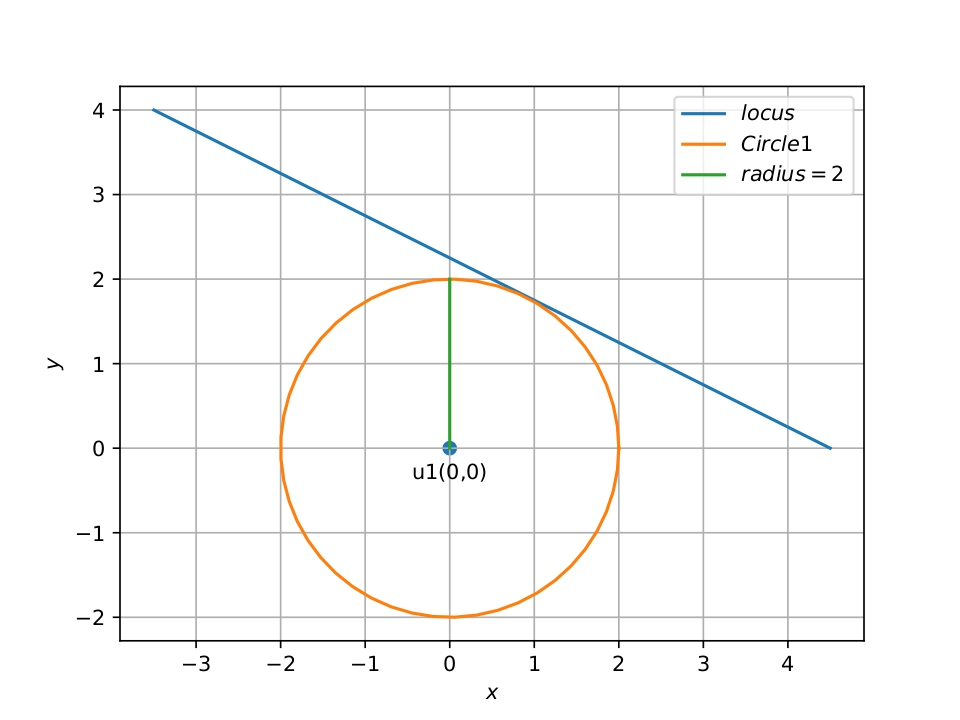
\includegraphics[width=\columnwidth]{fig.jpg}
    \label{fig:my_label}
    
\section{\textbf{Code Link}}

\begin{lstlisting}
https://github.com/sssurajit/fwc/blob/main/circle/codes/circle.py
\end{lstlisting}
Execute the code by using the command
\\ \textbf{python3 circle.py}
    



\end{document}

